% 
% Annual Cognitive Science Conference
% Sample LaTeX Paper -- Proceedings Format
% 

% Original : Ashwin Ram (ashwin@cc.gatech.edu)       04/01/1994
% Modified : Johanna Moore (jmoore@cs.pitt.edu)      03/17/1995
% Modified : David Noelle (noelle@ucsd.edu)          03/15/1996
% Modified : Pat Langley (langley@cs.stanford.edu)   01/26/1997
% Latex2e corrections by Ramin Charles Nakisa        01/28/1997 
% Modified : Tina Eliassi-Rad (eliassi@cs.wisc.edu)  01/31/1998
% Modified : Trisha Yannuzzi (trisha@ircs.upenn.edu) 12/28/1999 (in process)
% Modified : Mary Ellen Foster (M.E.Foster@ed.ac.uk) 12/11/2000
% Modified : Ken Forbus                              01/23/2004
% Modified : Eli M. Silk (esilk@pitt.edu)            05/24/2005
% Modified : Niels Taatgen (taatgen@cmu.edu)         10/24/2006
% Modified : David Noelle (dnoelle@ucmerced.edu)     11/19/2014
% Modified : Roger Levy (rplevy@mit.edu)     12/31/2018



%% Change "letterpaper" in the following line to "a4paper" if you must.

\documentclass[10pt,letterpaper]{article}

\usepackage{cogsci}
\usepackage{color}
\usepackage{graphicx}
\graphicspath{{figs/}}
%\cogscifinalcopy % Uncomment this line for the final submission 

\usepackage{tikz}
\usepackage{tikz-qtree}
\usepackage{subcaption}
\usepackage{pslatex}
\usepackage{apacite}
\usepackage{amsmath}
\usepackage{float} % Roger Levy added this and changed figure/table
                   % placement to [H] for conformity to Word template,
                   % though floating tables and figures to top is
                   % still generally recommended!

%\usepackage[none]{hyphenat} % Sometimes it can be useful to turn off
%hyphenation for purposes such as spell checking of the resulting
%PDF.  Uncomment this block to turn off hyphenation.


%\setlength\titlebox{4.5cm}
% You can expand the titlebox if you need extra space
% to show all the authors. Please do not make the titlebox
% smaller than 4.5cm (the original size).
%%If you do, we reserve the right to require you to change it back in
%%the camera-ready version, which could interfere with the timely
%%appearance of your paper in the Proceedings.

\providecommand{\tightlist}{%
  \setlength{\itemsep}{0pt}\setlength{\parskip}{0pt}}
  
\definecolor{Red}{RGB}{255,0,0}
\definecolor{Green}{RGB}{10,200,100}
\definecolor{Blue}{RGB}{10,100,200}

\newcommand{\mh}[1]{{\textcolor{Blue}{[mh: #1]}}}
\newcommand{\rl}[1]{{\textcolor{Green}{[roger: #1]}}}

\newcommand{\denote}[1]{\mbox{ $[\![ #1 ]\!]$}}
\newcommand{\red}[1]{{\textcolor{Red}{#1}}}

\title{Syntactic expectations modulate pragmatic interpretations of generic sentences}
 
\author{{\large \bf Michael Henry Tessler (tessler@mit.edu)} \\
  Department of Brain and Cognitive Sciences, MIT \\
  Cambridge, MA 02139 USA
  \AND {\large \bf Roger Levy (rplevy@mit.edu)} \\
  Department of Brain and Cognitive Sciences, MIT \\
  Cambridge, MA 02139 USA}


\begin{document}

\maketitle


\begin{abstract}

%A hallmark of human thinking is the ability to update our beliefs in the face of conflicting evidence. 
%Talk with the same person for long enough and you will be able to predict what they will say before they have said it.
%We investigate the interface between

Generic statements convey generalizations about categories, but  how a listener should generalize is not always clear.  
``Elephants live in Africa and Asia'' implies generalization across distinct subsets of the category (some live in Africa, others live in Asia).
Such conjunctive generics about mutually exclusive properties (e.g., , where each property applies to a distinct subset of the category) also pose interesting questions for theories of incremental processing because the meaning of the sentence can change part-way through. 
We extend a recently proposed computational model of generic language understanding with an incremental processing mechanism that makes novel predictions for partial interpretations of conjunctive generic sentences.
We test these predictions with two behavioral experiments. The results support a strong view of incrementality, wherein listeners  continuously use their expectations about where a speaker will go next with their utterance to update their beliefs.


%Generics permit exceptions (e.g., not all birds fly, and yet ``Birds fly'' is true) and adequately dealing with the exceptions is a problem for any model of generic language understanding. 
%Here, we examine an extreme case of exceptionality in generics: 
%We show how a recent model of generic language understanding that posits that the literal meaning of a generic is underspecified or uncertain can interpret conjunctive generics about mutually exclusive properties.  
%Furthermore, we extend this model to incorporate syntactic expectations about where a speaker will go next with her utterance.
%This joint syntactic--semantic/pragmatic model makes novel predictions for incremental interpretations of conjunctive generic sentences, which we test across three experiments.
%The success of this model highlights the deep connection between syntactic knowledge and pragmatic language understanding. 

\textbf{Keywords:} 
semantics; pragmatics; incremental processing; generics
\end{abstract}


\section{Introduction}

%Penguins would be upset if we understood the statement ``Birds fly'' to apply to the entire category of birds. 


Much of what we come to learn about the world comes not from direct experience but from knowledge conveyed to us from others, often in the form of linguistic utterances. 
``Elephants eat 300 pounds of a food in a day'' succinctly conveys information that extends beyond any particular moment in time or space (e.g., it could apply to any elephant, any day of the week). 
Utterances that communicate generalizations are called \emph{generic} utterances \cite{Carlson1977, genericBook}, and they are the foremost case study of rich, abstract knowledge conveyed in simple utterances \cite{Gelman2009}.

Generics are rife with philosophical puzzles that make it difficult to develop a unified, formal theory of their meaning \cite<for useful reviews, see:~>{genericBook, Nickel2016}.
One largely understudied puzzle concerns how generics combine.
To appreciate the complexity, consider the null hypothesis that generics to mean something analogous to a majority quantifier like \emph{most} or \emph{all} (e.g., ``Most elephants eat 300 pounds of food in day'').
How can such an account treat a generic about a conjunctive  property like ``Elephants live in Africa and Asia''? 
No elephant actually lives on both continents; instead, the sentence should be understood as ``Elephants live in Africa, and elephants live in Asia'', but this is impossible if each individual generic sentence means that the majority hold the property \cite<i.e., it is impossible for more than half of elephants to live in Africa and more than half of elephants to live in Asia;>{Nickel2008}.
This phenomenon is clearly the result of the interaction among the property: Learning about only one of the properties (e.g., ``Wugs live in Africa'') intuitively still conveys that most or all have the property. 
%\mh{Collective interpretation of ``all'', ``most'' doesn't run into the issues?}

The puzzle of understanding conjunctive generic sentences deepen when one considers that actual linguistic input is processed incrementally \cite<e.g.,>{Altmann1999}.: Listeners may start forming expectations about the intended meaning before the speaker finishes their sentence\cite<e.g.,>{rohde2011anticipating}.. 
For conjunctive generics about mutually exclusive properties,  incrementality in language understanding would imply non-monotonic reasoning: First, a listener believes that all elephants live in Africa (e.g., when they only hear that ``Elephants live in Africa''), and later believes that roughly half live in Africa (when the sentence completes ``...and Asia'').
Furthermore, a strong view of incrementality would predict intermediate degrees of belief (in how many elephants live in Africa) at the point of the sentence where a conjunct is introduced (at the ``and''). 
However, it is possible that human incremental processing mechanisms can only operate on meaningful content words, not function words like ``and''; such a theory would predict any interpretative difference between ``Elephants live in Africa'' and ``Elephants live in Africa and''. 

% but recent progress made been in developing a computational account for the meaning of generics \cite{Tessler2019:genLang}.

%Recent progress had been made, however, in developing a computational account for the meaning of generic langauge

%Understanding how generic language updates beliefs holds the key to understanding how young children build rich, intuitive theories \cite{Gelman2009}. 

%\mh{MH: don't attack cohen; instead stay at the level of the logical puzzle}
%One virtue of having a computational model of generic language is that it can make quantitative predictions about human behavioral data.

%\mh{incremental syntactic processes requires meaningful chunks}


%The sentence ``Robins lay eggs'' is true despite the property only applying to female robins, yet the same logic does not make ``Robins are female'' a true or felicitous utterance. 


%Crucially, this theory posits that the meaning of a generic is uncertain one which can be updated as more information is available.

%\mh{
%	we know XYZ, however it's an open question whether Z or Z'.
%	- incremental interpretation as one way in which we explore.
%	- right before expt. Model + Eq. 3 would imply X, but the facts of the world could be different.
%}

\begin{figure}
\centering
	\begin{subfigure}[b]{0.75\columnwidth}
	\centering
    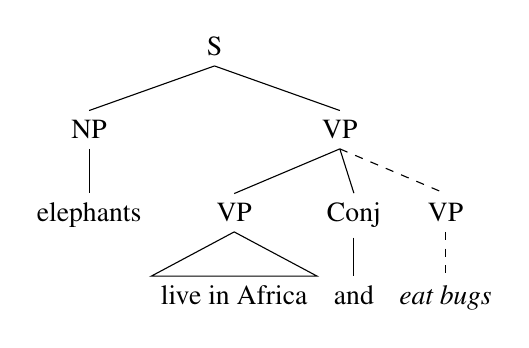
\begin{tikzpicture}[sibling distance=0pt]
	        \Tree [.S [.NP  elephants ]
	                  [.VP [.VP \edge[roof]; {live in Africa} ]
	                       	[.Conj and ] 
				\edge[dashed]; [.VP  \edge[dashed]; \emph{eat bugs}
				] ] ]
	\end{tikzpicture}
	    \caption{Parse 1}
\end{subfigure}%

\begin{subfigure}[t]{0.75\columnwidth}
\centering
	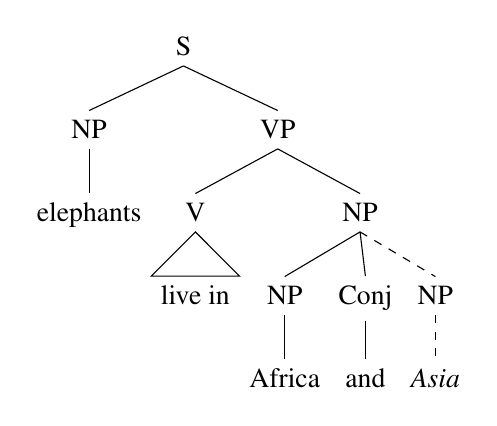
\begin{tikzpicture}[sibling distance=0pt]
	        \Tree [.S [.NP  elephants ]
	                  [.VP [.V \edge[roof]; {live in} ]
	                       	[.NP [.NP Africa ]
					[.Conj and ]
		                       	\edge[dashed]; [.NP  \edge[dashed]; \emph{Asia} ]] ] ]]
\end{tikzpicture}
    \caption{Parse 2}
   \end{subfigure}
   
\caption{Incremental syntactic trees corresponding to ``Elephants live in Africa and''}
\label{fig:trees}
\end{figure}

Recently, a computational model of generic language was proposed that makes quantitative predictions about human behavioral data \cite{Tessler2019:genLang}.
In addition to making quantitative predictions, a computational language understanding model can integrate rather seamlessly with probabilistic models of syntactic processing \cite{Levy2008} and generate predictions about incremental understanding.
In this paper, we do just this. 
We test the novel predictions of this model in two behavioral experiments that probe listeners' understanding of conjunctive generic sentences at different points in a sentence, analogous to gating paradigms in psycholinguistics \cite{Grosjean1980}.
We find that the strongest view of incremental processing is supported.
 
%Here, we combine a recent model of generic language understanding  \cite{Tessler2019:genLang} with an incremental parsing mechanism to begin to form beliefs about a speaker's intended meaning before the speaker has finished speaking.
%The basic, non-incremental model understands ``Elephants live in Africa and Asia” as meaning that some elephants live in Africa and that different ones live in Asia, in the case where listeners have prior knowledge suggesting against the existence of elephants that live on both continents (\emph{international elephants}).
%Furthermore, the enriched incremental model makes the prediction that part-way through generic sentences about conjunctive predicates (e.g., ``Elephants live in Africa''), a listener will form strong beliefs (i.e., \emph{all elephants live in Africa}) which later get non-monotonically updated once more information comes in (\emph{some live in Africa and some live in Asia}).
%A model that allows for full interactions between the levels of syntactic processing and pragmatic reasoning allows for even finer-grained interpretations. 
%We test such a model in a set of language understanding tasks where participants are asked to report their beliefs about the prevalence of a property in a category at different points in a sentence, analogous to gating paradigms in psycholinguistics \cite{Grosjean1980}.


%Recently, \cite{Tessler2019:genLang} proposed a theory of generic language wherein the meaning of a generic is \emph{underspecified} (or, vague) and Bayesian reasoning is used to resolve more precise meanings in context.


%Intriguingly, this model also predicts that (i.e., upon hearing only that ``Elephants live in Africa'') leads our model to believe that most, possibly all, elephants live in Africa, but when the sentence is completed (``. . . and Asia''), the model nonmonotonically updates its beliefs to the weaker \emph{some elephants live in Africa and others in Asia}. 


%Interpreting generics in a consistent way is a non-starter. 


%Theories that appeal to standard, formal semantic, quantificational truth conditions (e.g., generic means \emph{most} or \emph{all} relevant or normal members of the category have the property) employ mechanisms to implicitly restrict the \emph{relevant} set of robins to be females in the case of a property concerning reproduction such as \emph{laying eggs}\cite<e.g.,>{Cohen1999}. 
%(such as that of  where a generic ``Ks F'' means roughly that \emph{most of the relevant Ks F})

%Interpreting generics in a 
%Such restrictions, however, are too limiting when interpreting conjunctive predicates as in ``Elephants live in Africa and Asia''. 
% from knowledge about the kind of property under consideration (i.e., \emph{laying eggs} has to do with reproduction, so we are only talking about females), but this mechanism is too restrictive when it comes to generics about conjunctive properties such as ``Elephants live in Africa and Asia'': 
%It cannot be the case that most (more than half of) elephants live in Africa and most (more than half of) elephants live in Asia, unless we imagine elephants migrating back-and-forth from continent to continent (i.e,. \emph{international elephants}), which is intuitively implausible \cite{Nickel2008}.
%More generally, a theory of generics need be sufficiently flexible to accommodate property-specific interpretations (e.g., ``Robins lay eggs'' means half of robins lay eggs; ``Dogs get cancer'' means some dogs get cancer; ``Birds fly'' means almost all birds fly) as well as be able to revise those interpretations with new, potentially conflicting evidence (e.g., consider ``Elephants live in Africa''~vs.~``Elephants live in Africa and Asia'').



%``Lions have manes and give live birth'' wherein the first and second conjuncts apply to distinct subsets (i.e., male lions have manes and female lions give live birth).



%Consider the following examples:
%
%\begin{enumerate}
%\tightlist
%\item Triangles have three sides and three angles.
%\item Ravens have two wings and two legs.
%\item Elephants live in Africa and Asia.
%\item Lions have manes and give live birth.
%\end{enumerate}
%
%It is conceivable that both (1) and (2) can be analyzed in terms of a (context-sensitive) generic operator acting on a logically complex predicates (i.e., \emph{all triangles both have three sides and three angles}, \emph{most ravens have two wings and two legs}). 
%Individual elephants do not migrate across continents and thus live in both Africa and Asia. 
%The individual lions that have manes are a distinct sub-category from those that give live birth (i.e., the properties pick out the males and the females, respectively). 
%The logically complex predicates in sentences (3) and (4), thus, are not true generically of their associated categories; rather, the sentences should be understood as a conjunction of generic sentences.

\section{Computational Model}

We extend the generic interpretation model of \citeA{Tessler2019:genLang} to incorporate an incremental processing mechanism that allows a listener to understand meaningful chunks of a full utterance.
The basic model interprets a generic utterance predicating a property of a category (``Elephants eat 300 pounds of food in a day'') as meaning that the \emph{prevalence} $x$ or probability of the property given the category---$P($eats 300 lb. of food in a day$\mid$ is an elephant$)$---is greater than an \emph{a priori} uncertain threshold $\theta$.
The literal meaning of the generic---an uncertain threshold function---combines with a listener's prior knowledge about the prevalence of the feature $P(x)$ within a relevant set of alternative categories (e.g., other animals) to compute a posterior distribution over prevalence $x$. 
\begin{equation}
P(x \mid u) = \int_{\theta} P(x, \theta \mid u)  d\theta \propto P(x) \cdot P(\theta) \cdot \delta_{\denote{u}(x, \theta)} 
\label{eq:L0}
\end{equation}
\noindent where $\delta_{\denote{u}(x, \theta)}$ is the Kronecker delta function assigning a value of 1 for utterances that are literally true (in the case of a generic: where $x > \theta$) and 0 for utterances that are false.

Equation \ref{eq:L0} is a model of a Bayesian listener interpreting a generic utterance.
To interpret a generic about a conjunctive predicate, there are two possibilities:

\begin{equation}
\begin{split}
[G_\theta x. \textnormal{ elephants}(x)& \to \textnormal{live\_in}(\textnormal{Africa})] \land \\
[G_\theta x. \textnormal{ elephants}(x)& \to \textnormal{live\_in}(\textnormal{Asia})] 
\end{split}
\label{eq:sem}
\end{equation}

\begin{equation}
[G_\theta x. \textnormal{ elephants}(x) \to \textnormal{live\_in}(\textnormal{Africa} \land \textnormal{Asia})]
\label{eq:sem1}
\end{equation}

The model can interpret multiple generics in succession, using the posterior distribution over prevalence $P(x \mid u)$ as the prior for the next utterance. 
Take our running example of ``Elephants live in Africa and Asia''.


We start with a joint prior over the prevalence of the two properties: $P(\vec{x}) = P(x_{Af}, x_{As})$, which we incrementally update with each successive generic. 

\begin{eqnarray}
P(\vec{x} \mid u_{Af}, u_{As})& \propto & P(\vec{x}, \vec{\theta} \mid u_{Af})  \cdot \delta_{\denote{u_{As}}(x_{As}, \theta_{As})} %\\
%		& \propto & P(\vec{x}) \cdot P(\vec{\theta}) \cdot \delta_{\denote{u_{Af}}(x_{Af}, \theta{Af})} 
\label{eq:L0a}
\end{eqnarray}
\noindent where $P(\vec{x}, \vec{\theta} \mid u_{Af})$  is the posterior that results from Eq.~\ref{eq:L0}.
The predictions for a sequential understanding of ``Elephants live in Africa and Asia'' are shown in Figure \ref{fig:model}.

In addition to processing multiple utterances, listeners may begin to form expectations about the complete utterance even before the sentence is over. 
For example, in the case of interpreting a generic sentence about a conjunctive property (e.g., ``Elephants live in Africa and Asia''), a listener is given the opportunity to form a partial, plausible interpretation of the utterance by the time they read the first conjunct (``Africa''). 
In order to model incremental interpretations of the utterance, we extend this model to allow a listener to form expectations about plausible continuations from sentence fragments $f$.
To do this, we assume that a listener has probabilistic expectations about how a speaker will choose to complete the utterance given a fragment $P(u' \mid f)$.

\begin{equation}
P(x \mid f) = \sum_{u'}) P(x \mid u') P(u' \mid f) 
\label{eq:L0a}
\end{equation}

We consider the case of listeners encountering the coordinating connection ``and'' in the predicate of a generic sentence. 
For simplicity, we assume that speakers can continue a sentence such as ``Elephants live in Africa and'' with either an NP coordination with a mutually exclusive property (``Asia'') or VP coordination with a non-mutually exclusive property (``eat 300 pounds of food a day'').\footnote{
	Of course, NP-coordination with non-mutually exclusive properties is possible (e.g., ``eat figs and nuts''). 
	Our focus in this paper is on the fact that a speaker can continue the conjunction with a mutually exclusive or non-mutually exclusive property, which in the cases we consider, are perfectly correlation with NP~vs.~VP coordination.
}

\begin{figure}[h]
  \centering
    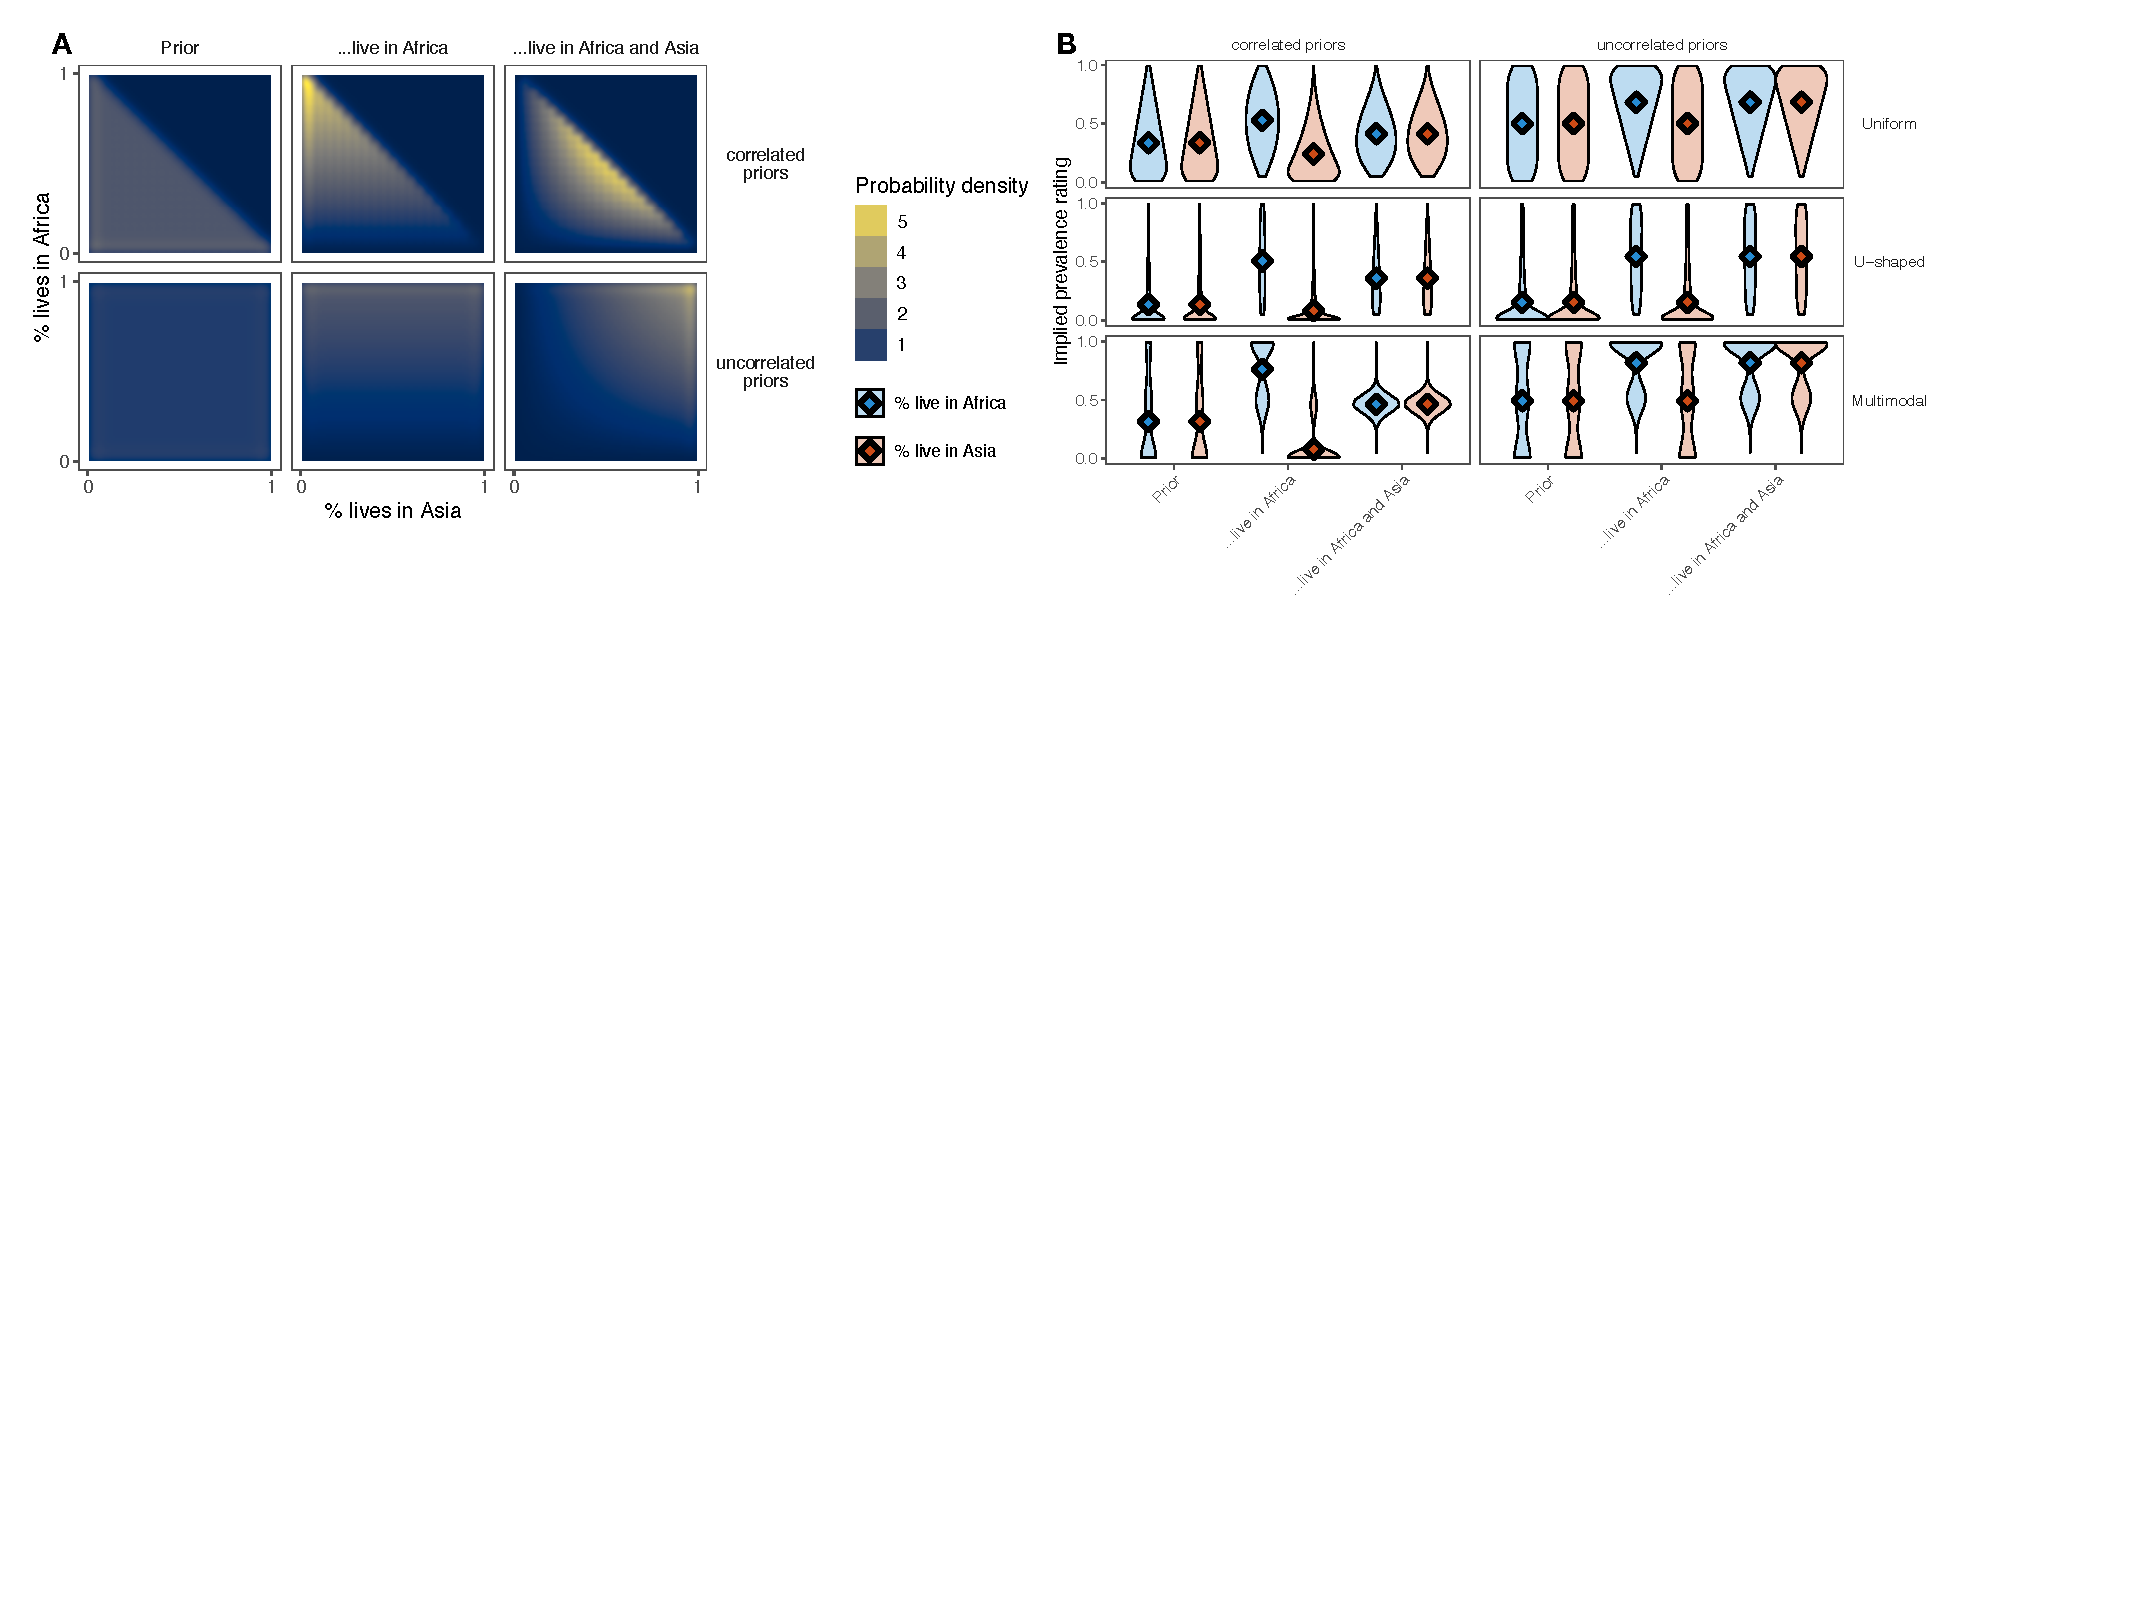
\includegraphics[width=0.5\textwidth]{model}
%    \vspace{-1cm}
  \caption{
  \red{Replace with figures of joint distributions, plus ``hard-core incremental'' predictions}
  Model interpretation of a conjunctive generic (``Elephants live in Africa and Asia''). A: Intuitive priors for marginal distributions of prevalence for living in Africa and living in Africa. B: Partial interpretation upon hearing utterance (“Elephants live in Africa . . .”). C: Full interpretation upon hearing the end of the sentence (``...and Asia''). Uncertainty about the threshold for generic sentences allows the listener to non-monotonoically update its beliefs about the prevalence of the feature in categories.
  }
  \label{fig:model}
\end{figure}



%Extending an analysis of generics to handle complex-predicates poses unique challenges.
%A sentence of the form ``Ks F and G'' introduces an ambiguity:
%
%\begin{enumerate}
%\tightlist
%\item $\denote{gen}(K) [F \land G]$
%\item $\denote{gen}(K) [F] \land \denote{gen}(K) [G]$
%\end{enumerate}


\section{Experiments}

We design three experiments to test the mutual exclusivity (ME) and incremental predictions of the model. 
Experiment 1 tests the basic ME predictions that ``Elephants live in Africa and Asia'' means roughly that half live in Africa and half live in Asia; we compare interpretations for these conjunctive generics with those of conjunctive generics about non-mutually exclusive (NME) properties (e.g., ``Elephants live in Africa and eat 300 lb. of food in a day''). 
Experiment 2 is a conceptual replication using an adaptation of a gating paradigm \cite{Grosjean1980} which also controls for asking about two properties previously mentioned using a conjunctive generic sentence. 
Experiment 3 uses the gating paradigm to test the fine-grained incremental predictions of the model.
%Sample size, participant exclusion criteria, and primary planned analyses for all experiments were pre-registered on OSF \red{(url removed for blinding)}.


\begin{figure*}[h]
  \centering
    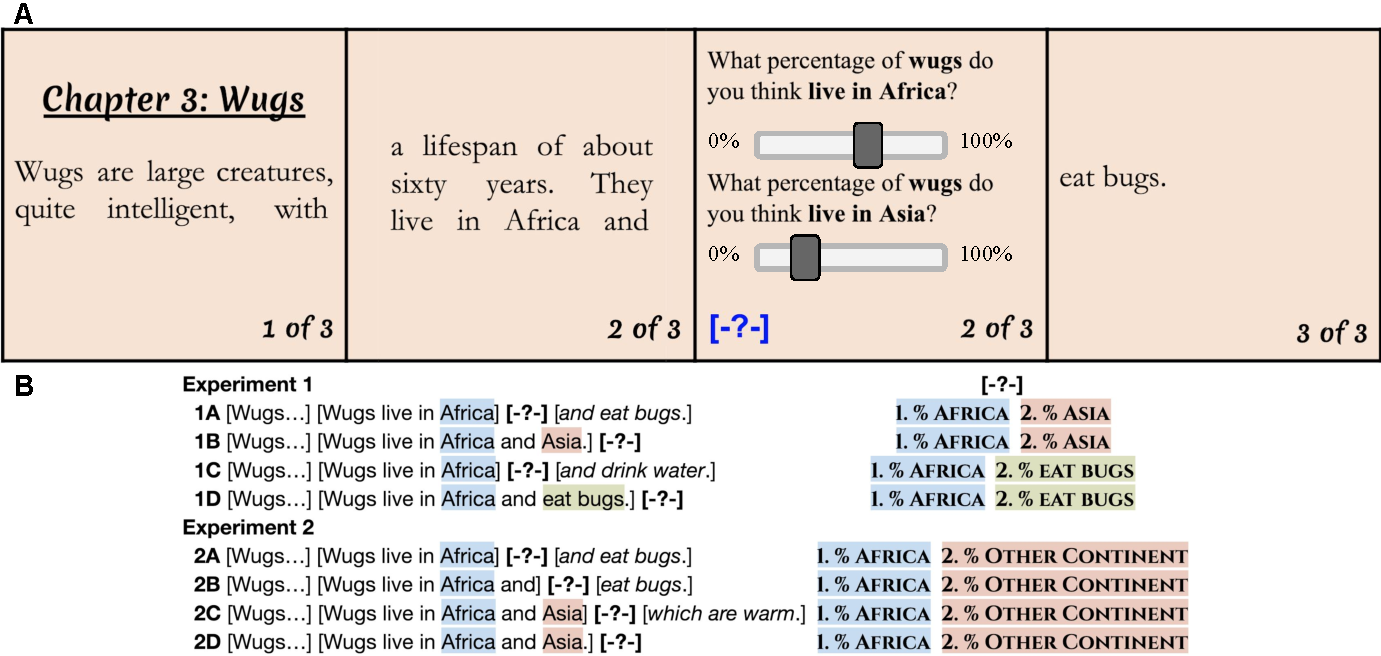
\includegraphics[width=1\textwidth]{design}
%    \vspace{-1cm}
  \caption{\red{Make clearer and more beautiful?} \mh{replace example with sample chapter}Overview of experiments. Experiment 1 compared interpretations of generics about mutually exclusive (ME) properties and non-mutually exclusive properties (NME), by asking about the implied prevalence of the two ME properties. Experiment 2 queried for partial interpretations of conjunctive generics by interrupting with a question ([-?-]) after the first property;  in addition, Expt. 2 measure implied prevalence for the two NME properties (e.g., \% eat bugs). Experiment 3 queried for partial interpretations by interrupting at three different points in the sentence. }
  \label{fig:expt1}
\end{figure*}

\subsection{Experiment 1}

%\subsubsection{Methods}
\subsubsection{Participants}
We recruited \red{N} participants through Amazon's Mechanical Turk.
This number was arrived at with the aim of collecting \red{N} participants' data who passed the attention checks.  
Participants were restricted to those with verified U.S. IP addresses and had at least a 95\% work approval rating. 


\subsubsection{Materials}

Participants read a storybook concerned with aliens and animals on a far-away planet.
% without any larger narrative (each chapter concerned different categories or characters).
Stimuli consisted of \red{16} unrelated paragraphs of text called \emph{chapters}, which contained between 2--4 sentences, broken up across between 2--4 screens.
Each chapter ended with a generic sentence about conjunctive properties, which differed only in whether the second property was mutually exclusive (ME) with the first (\emph{conjunct type}): ``Glippets live on the southern continent of Caro and \emph{on the northern continent of Este (ME) /  enjoy the sunshine there (nME).}''
The preceding content of the chapter was either unrelated to these properties or supported the mutually exclusive interpretation of the properties in the case that the properties were not \emph{ipso facto} mutually exclusive (e.g., ``Krens are a tribe of the aliens that live on the continent of Benli, which has no agriculture. Animals like stups, four-legged creatures with large antlers, are a resource for the Krens. Stups roam all over the windy highlands of Benli, far from the oceans. Krens are stup-herders and \emph{fisherman} / \emph{incorporate stups into their religion}.'')

Conjunct type was manipulated within-participants and within-items. 
In addition to the experimental items, the storybook included \red{N} filler chapters, which concerned similar content to the experimental chapter but which asked about properties that were described with explicit quantifiers such as \emph{most}, \emph{all}, or \emph{none}. 

%We used \red{10} critical chapters (items), each which could be assigned to one of two experimental conditions.
%A given chapter in the two experimental conditions differed only in the information present on the final screen of a chapter.
%The penultimate screen of all critical trials ended with the beginning of a conjunctive sentence that was broken up immediately before the ``and'' in the sentence \red{(Figure); e.g., ``They ascribe to the Caboo religion'')}. 
%Text on the page was fully-justified so that the final word on a page always appeared in the bottom-right corner of the screen, giving the appearance that the page naturally ended at that word.
%In the \emph{relevant conjunction} condition, the continuation of the sentence (final screen) was a property that was anti-correlated (or, somewhat mutually exclusive) with the property on the preceding page (e.g., ``and the Daith religion''). 
%In the \emph{irrelevant conjunction} condition, the continuation was a property that was unrelated to the property on the preceding page (e.g., ``...and follow a strict code of laws.''). 
%In addition, we had 5 filler trials which appeared similar to the \emph{irrelevant conjunction} cases.

\subsubsection{Procedure}
Participants were told they would be reading a storybook and be asked questions at the end of each chapter. 
Questions were all of the same type, an \emph{implied prevalence} question \cite{Gelman2002, Cimpian2010} that read: ``What percentage of Ks do you think F?'', where K represents a category and F a feature. 
Responses were recorded using a 101-pt slider bar with end-points labeled 0\% and 100\%, and with the exact value selected appearing above the slider. 
Participants were familiarized with the response variable in a practice trial, where they were asked to report how many dogs bark, birds are male, cats get cancer, and lions lay eggs. 
We used these questions to encourage participants to use the full range of the response scale. 



Following this instructions and practice questions, participants read the storybook.
% consisting of \red{16} paragraphs we refer to as \emph{chapters} (items), each of which spanned 2 - 4 screens of text which spanned 2 - 4 lines on the screen. 
At the end of each chapter, participants answered a pair of implied prevalence questions relating to information present in the chapter. 
For critical trials (both mutually exclusive and non-mutually exclusive conjunct types), the questions asked about the two mutually-exclusive properties.
For filler trials, the two questions were asked about two properties that were conveyed using the same quantifiers (i.e., properties both described with \emph{all}, \emph{most}, or \emph{none}).
At the end of the storybook, participants completed a memory check question where they had to select all the facts they had learned in the story from a list of 10 (5 real, 5 distractor); in addition, participants were asked to explain, in very broad terms, what the experiment was about.

%The text of a chapter mostly composed of generic sentences about novel categories (e.g., ``Glippets are intelligent creatures''), though some sentences mentioned specific fictional characters (``Wint lived a long time ago in the mountains.'').

%Eaach chapter of the storybook was on

\paragraph{Results and discussion}

\begin{figure}[h]
  \centering
    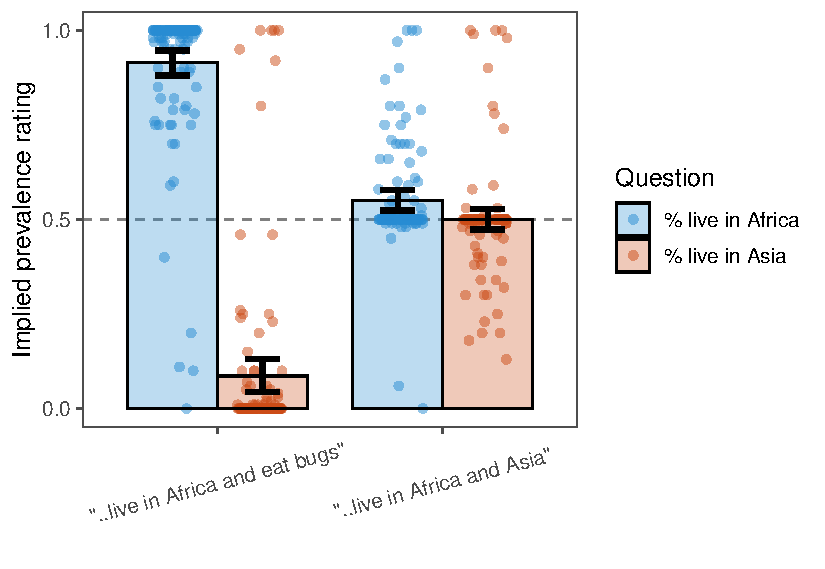
\includegraphics[width=0.5\textwidth]{expt1_summary}
%    \vspace{-1cm}
  \caption{Experiment 1 results. Participants' ratings of the percentage of a category with a property (color) upon hearing a conjunctive generic either with non-mutually exclusive properties (left) or mutually exclusive properties (right). Error-bars denote bootstrapped 95\% confidence intervals; points are individual responses. \mh{does mutual exclusivity fail for some people?}}
  \label{fig:expt1}
\end{figure}




\red{N} participants were excluded for either failing to respond accurately to all of the practice trials, failing to respond accurately to at least 7 of the 10 memory check prompts (same exclusion criteria for all experiments), or responded randomly to the explanation question in a way that suggested they were a bot (e.,g., ``nice experiment'' in all caps; often if they failed the explanation trial, they failed at least one of the two other checks). 
Our primary analysis is whether implied prevalence estimates to the first property in a conjunctive generic sentence (e.g., the \% of elephants that live in Africa) changes as a function of the second property.
In particular, we predict that implied prevalence estimates for the first conjunct will be higher when the second conjunct is not mutually exclusive than when it is ME. 
To test this prediction, we constructed a Bayesian mixed-effects regression model predicting implied prevalence ratings to the first conjunct (e.g., \% live in Africa) as a function of the second conjunct that appeared in the sentence.
%\footnote{
% We model the raw data as being generated from a 0- and 1-inflated beta distribution. This allows us to keep the data in a raw format (as %slider bar ratings between 0-1, including the endpoints).
%}
In addition, we included by-item and by-participant random-effects of intercept and effect of condition manipulation.
Consistent with our prediction, participants responded that substantially fewer elephants lived in Africa when they read ``Elephants live in Africa and Asia'' then when they read ``Elephants live in Africa and eat 300 lb. of food a day'' (posterior mean estimate and 95\% credible interval: $\beta = -2.11 [-1.2, -3.3]$; Figure \ref{fig:expt1}).  

\subsection{Experiment 2: Interrupting questions}

In Expt.~1, we observed that the nature of the second conjunct in a conjunctive generic sentence can influence inferences about the prevalence of the first conjunct.
Here, we test for a potential confound in the design of Expt.~1: Whenever participants provided prevalence estimates for two properties that they had read about in a conjunctive generic, the inference was that they were mutually exclusive. 
Here we provide a control wherein participants can provide ratings about two properties previously mentioned in a conjunctive generic but which are not  mutually exclusive. 
In addition, we aim to replicate the pattern of Expt.~1 using a gating technique wherein participants are queried part-way through a sentence. 

\subsubsection{Participants}

We recruited \red{N} participants through Amazon's Mechanical Turk.
This number was arrived at with the aim of collecting \red{N} participants' data who passed the attention checks.  
Participants were restricted to those with verified U.S. IP addresses and had at least a 95\% work approval rating. 

\subsubsection{Materials and procedure}

The materials were the same as used in Expt.~1 and the procedure was identical except for the critical trials.
Each critical trial either had a question at the end of the chapter (as in Expt.~1; \emph{uninterrupted condition}) or immediately before the final page of the chapter (\emph{interrupted condition}).
For the interrupted conditions, the critical sentence broke at the page-break before the conjunction (e.g., ``Elephants live in Africa\_\_'', where \_\_ denotes the page break). 
For the uninterrupted conditions, the question appeared at the end of the chapter.
Each chapter ended with a generic sentence about conjunctive properties, which differed only in whether the second property was mutually exclusive (ME) with the first (\emph{conjunct type}): ``Glippets live on the southern continent of Caro and \emph{on the northern continent of Este (ME) /  enjoy the sunshine there (nME).}''

%E2: AF&AS / AF/  AF&NME[Qnme] / AF[Qnme]
\begin{figure}[h]
  \centering
    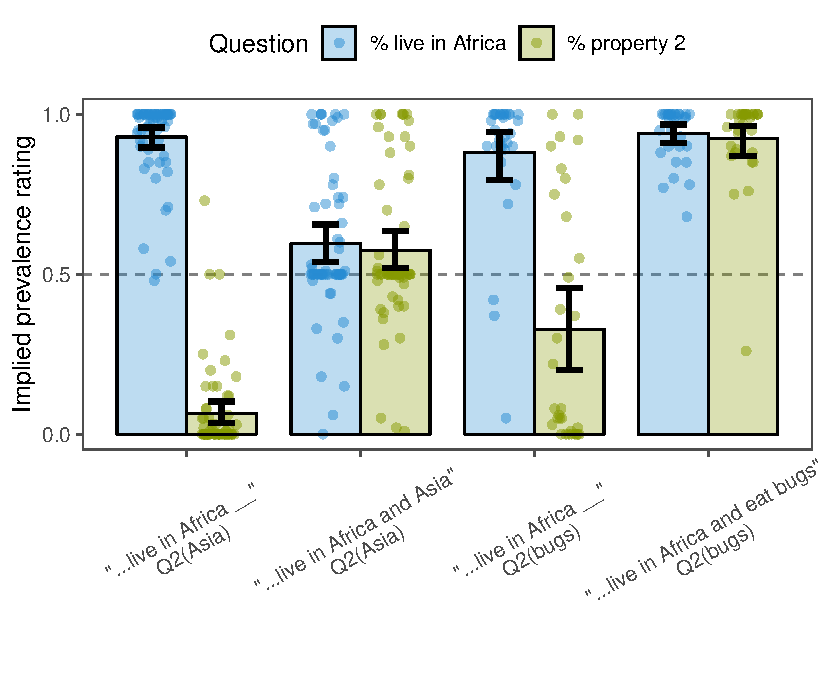
\includegraphics[width=0.5\textwidth]{expt2_summary}
%    \vspace{-1cm}
  \caption{Experiment 2 results.  Participants rate prevalence for mentioned property (\% live in Africa) and ``Property 2'', either the mutually exclusive property (left two bars) or non-mutually exclusive property (right two bars). ``\_\_'' indicates the question appears mid-sentence.}
  \label{fig:expt2}
  \end{figure}


\subsubsection{Results}

These results replicated the findings of Expt.~1 using an interrupting question and shown that the results cannot be attributed to asking about two properties mentioned in a conjunctive generic sentence. Hearing only that ``Elephants live in Africa\_\_'' led listeners to believe that all elephants lived in Africa (Figure \ref{fig:expt2} left-most bars), whereas if the sentence finished ``\_\_and Asia'', listeners inferred that roughly half live in Africa and half live in Asia. The same is not true for properties that are not construed as mutually exclusive (Figure \ref{fig:expt2} right-most bars), where the generic is thought to apply strongly to both properties. 
\mh{3rd condition in expt 2 is the prior}

\subsection{Experiment 3: Interrupting questions}

In Expt.~2, we replicated the mutually-exclusive inference effects of Expt.~1 using a gating paradigm wherein participants are queried for their beliefs part-way through a sentence. 
Here, we exploit this paradigm to test the incremental processing predictions of the model, wherein syntactic expectations can modulate the interpretations of generic sentences in a fine-grained manner. 

\subsubsection{Participants}

We recruited \red{N} participants through Amazon's Mechanical Turk.
This number was arrived at with the aim of collecting \red{N} participants' data who passed the attention checks.  
Participants were restricted to those with verified U.S. IP addresses and had at least a 95\% work approval rating. 

\subsubsection{Materials and procedure}

The materials were modeled on the materials from Expts.~1\&2, but were modified to explicitly introduce both ME properties early in the chapter (e.g., ``Kweps live in forests made up of xorfun trees and tunkel trees... Kweps chew on the bark of xorfun [and tunkel]'').
In addition, we added filler trials to increase the frequency with which ME properties were predicated of categories; these took the form of the critical trials from Expt.~1 where ME properties were described of a category and questions concerning the ME properties appeared at the end of the chapter. 
In addition, these half of these filler trials had page breaks immediately before the ``and'' and half immediately after.

On critical trials, questions appeared in the middle of the chapter. 
There were three kinds of critical trials, which determined where the page break (and hence, question) occurred in the conjunctive generic sentence: after ``Africa'', after ``and'', or after ``Asia''. 
When participants did not see the full conjunctive property (e.g., ``Africa and Asia''), the sentence continued after the question with a non-mutually exclusive property (e.g., ``Africa and eat bugs''), so as to not give the impression that the participant was being tricked. 


 \subsubsection{Results}
\begin{figure}[h]
  \centering
    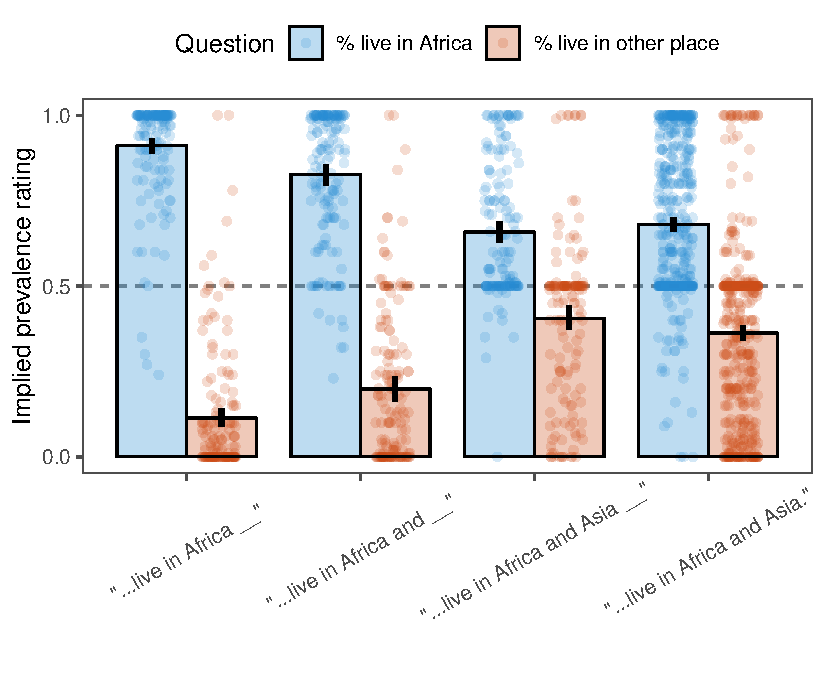
\includegraphics[width=0.5\textwidth]{expt3_summary}
%    \vspace{-1cm}
  \caption{Experiment 3 results. Participants are interrupted at various stages of the sentence (either after \emph{Africa}, \emph{and}, or \emph{Asia}) to be asked about the prevalence of \emph{living in Africa} and \emph{living in Asia}, or asked at the end of the sentence (right-most bars). When participants are interrupted before the second conjunct (\emph{Asia}), the sentence continues with a non-mutually exclusive property.}
    \label{fig:expt3}
  \end{figure}
  
 \mh{Expt 3: 
 - ``live in Africa.'' condition?
 - ``live in Africa.'
 }
 

\red{N} participants were excluded for either failing at least one of the three attention checks.
We find that the participants' implied prevalence ratings of how many elephants lived in Africa monotonically decreased as a function of how many words of the conjunctive predicate they were allowed to see. 
When participants learned that ``Elephants live in Africa and Asia'', they tended to infer that it was half that lived in Africa and half in Asia.
If participants only read that ``Elephants live in Africa'', they tended to infer that significantly more lived in Africa. 
Crucially, if participants saw that the sentence had a conjunction (``Elephants live in Africa and''), their inferences about the implied prevalence of living in Africa was in between the two others (Figure \ref{fig:expt3}).

\begin{table*}[!htb]
\begin{tabular*}{\textwidth}{p{5cm}|p{6cm}|p{6cm}}
Property & Mutually Exclusive (ME) & Non-Mutually Exclusive (NME) \\ \hline
ascribe to Cabooism & ascribe to some other religion & pray three times a day \\ 
live on the continent of Caro & live on some other continent & graze on the tall grasses \\ 
have territories at the tops of tall mountains & have territories in other geographical locations & watch over the low-lying regions during the day \\ 
plant fujusi & plant some other crop & spray their fields with a naturally-occurring fertilizer \\ 
build nests in gluers & build nests in other places & store tree-bark in them for safe keeping \\ 
are stup-herders & do something else for a living & sing songs to the stups to help them relax \\ 
have long wings & have some other type of wing & have sharp claws \\ 
wear wutsats around their heads & wear something else around their heads & carry sticks with them \\ 
chew on xorfun bark & chew on some other kind of bark & jump up and down in circles \\ 
carry their young in guklags & carry their young in something else & are very protective \\ 
are part of the Tinnoclan & are part of some other guild & sell their baskets in the Warfi marketplace \\ 
hibernate in fallen logs & hibernate in some other location & give birth twice a year \\ 
has bumpy skin & has some other-textured skin & produce fruit with a sour taste \\                                     
\end{tabular*}
\caption{Stimuli}
\end{table*}


\section{Discussion}

Generic sentences exhibit extreme sensitivity to context that make it difficult to precisely define what a single generic conveys. 
``Elephants live in Africa and Asia'' means neither that \emph{most elephants live (in both) Africa and Asia} nor that \emph{Most elephants live in Africa, and most elephants live in Asia}.
Here, we build on the observation of \citeA{Nickel2008} that the range of troubling examples for quantificational views of generics is quite large by empirically measuring interpretations of generics about conjunctive predicates.  
Notably, the uncertain threshold model of \citeA{Tessler2019:genLang} accounts for these examples seamlessly: An underspecified semantics can be updated as more information comes in. 

It is largely agreed that the context-sensitivity of generics needs to be accounted for at the level of individual properties in a particular context \cite{Nickel2008, Nickel2016, Sterken2015} as opposed to a purely more general framework where generics about different kinds of properties get ascribed different meanings \cite<e.g.,>{Prasada2013, Leslie2008}.
Here we show that in fact the same property (``lives in Africa'') can be understood in two different ways when presented in a generic sentence. 
When listeners hear that ``Elephants live in Africa'', they tend to think all elephants live in Africa; when they hear that ``Elephants live in Africa and Asia'', the implied prevalence of those living in Africa is quite lower. 
This phenomenon bears some similarity to the \citeA{Nickel2008}'s ``Dobermans have pointy ears'', which in a context of dog-breeders is entirely acceptable, but not so in a discussion of dog genetics (Dobermans are born with floppy ears and breeders clip their ears to make them pointy).
The unifying thread is that the same generic sentence can have dramatically different interpretations depending on the context. 
Thus, the work here moves us one step closer to developing a unified treatment of the ways in which context can affect the meaning of generics.

The uncertain threshold model of \citeA{Tessler2019:genLang} models the interpretation of conjunctive generics about mutually exclusive properties such as ``Elephants live in Africa and Asia'' as incrementally updating the threshold beyond which the property holds (generically) in the category (see Model Predictions). 
The model interprets the sentence as the conjunction of two full-blown generic sentences (``Elephants live in Africa, and elephants live in Asia''). 
This phenomenon, however, appears as the inverse of the Free Choice effect, wherein listeners apply a conjunctive interpretation (``and'') to a disjunction (``or''), as in ``You can have ice cream or cake''. 
Thus, an alternative account to the incremental, threshold updating model proposed here is that conjunctive generics about ME properties are the result of a similar kind of pragmatic inference one would use for the Free Choice account. 
One way to potentially disambiguate the reverse-Free Choice from the incremental threshold updating model would be to investigate quantifier sentences which have a fixed-meaning (e.g., ``Most'' means roughly more than half).
Naturally occurring examples of this sort exist (e.g., ``Elephants are beautiful, gentle giants that we are viciously taking away from this world. They are the largest land animal on Earth and are one of the gentlest creatures. Most live in Africa and Asia but are brought to other places for the entertainment of humans.'')\footnote{
Example from \url{https://www.theodysseyonline.com/want-to-ride-an-elephant}
} but further work is needed to determine the felicity and interpretation of such utterances.

In Expt.~3, we manipulated syntactic expectations by providing both additional information about the two mutually exclusive properties as well as additional fillers which contained conjunctive generics about ME properties. 
We find suggestive evidence that syntactic expectations can guide incremental pragmatic understanding of generic sentences. 
This calls for more tight-coupling between models of syntactic processing \cite{Levy2008} and pragmatic language understanding \cite{Goodman2016}. 
Methodologically, it is possible that either one of our context manipulations (e.g., highlighting two salient properties to participants) would be sufficient to impact listeners' syntactic expectations for continuations of conjunctive predicates.
It is also an open question what are listeners' baseline levels of syntactic expectations about conjunctions in these environments. 
%We are also actively investigating participants' baseline level of syntactic expectations using a cloze test.






\section{Acknowledgments}

We thank Karen Gu for her assistance in stimuli creation and experiment implementation.


\bibliographystyle{apacite}

\setlength{\bibleftmargin}{.125in}
\setlength{\bibindent}{-\bibleftmargin}

\bibliography{elephants}


\end{document}
